\section{Bit of  Differential Geometry: Dayuum!!}
Let us look into a bit of differential geometry which is a formal way of treating this tensor thingy. We will try to be as intuitive and non-rigorous as possible (and thus increasing our chances of making a mathematician crazy!) but yeah, we will try to be rigorous enough so that I am satisfied.
\subsection{Some prior things}
Before touching manifolds, let us define what an abstract topological space is, since manifolds are special case of topological spaces. 
\begin{definition}[Topological Space]
  A topological space is a set $(X, \uptau )$ where $\uptau \subset \mathcal{P}$ is a collection of subsets of $X$ such that:
\begin{itemize}
    \item $\emptyset, X \in \uptau$.
    \item $U_\alpha \in \uptau \implies \bigcup \limits_{\alpha\in J} U_\alpha \in \uptau$  (closed under arbitrary union).
    \item $U_i \in \uptau \implies \bigcap \limits_{i=1}^n U_i \in \uptau$  (closed under finite intersection)\footnotemark.
\end{itemize}
\end{definition}
\footnote{Here $\alpha$ index is used when we want the indexing set $J$ (indexing set means the set from where the incides to denote the elements of the set are taken from) to be arbitrary, meaning that the set $\{U_\alpha\}$ can be finite, countable or uncountable. On the other hand, index $i$ is mostly used when the indexing set is finite.}

Well well, this does not look anything like coffee cup and donut which most people associate topology with. That is a case of \textit{homeomorphism} which will be discussed later (hopefully). However, for now let us proceed. The sets belonging to $\uptau$ are called \textbf{open sets}. We define a \textbf{closed set} as a set whose complement is open. There are umpteen other definitions like \textbf{closure, boundary, interior, neighbourhood}, etc. Let define few of them \emoji{loudly-crying-face}. 
\begin{itemize}
    \item \textit{Closure} of a set $A$ is the smallest closed set containing $A$ and is denoted by $\overline{A}$.
    \item \textit{Interior} of a set $A$ is the largest open set contained in $A$ and is denoted by $\text{int}(A)$.
    \item \textit{Boundary} of a set $A$ is the set of points which are neither in the interior nor in the exterior of $A$ and is denoted by $\partial A$.
    \item If $p\in X$, then a \textit{neighbourhood} of $p$ is a set $N$ such that there exists an open set $U\in \uptau$ with $p\in U\subseteq N$.
\begin{figure}[H]
      \centering
      

\tikzset{every picture/.style={line width=0.75pt}} %set default line width to 0.75pt        

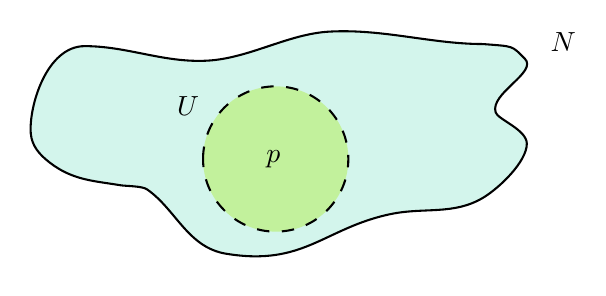
\begin{tikzpicture}[x=0.75pt,y=0.75pt,yscale=-1,xscale=1]
%uncomment if require: \path (0,203); %set diagram left start at 0, and has height of 203

%Curve Lines [id:da28281619681811754] 
\draw [fill={rgb, 255:red, 211; green, 245; blue, 236 }  ,fill opacity=1 ][line width=0.75] [line join = round][line cap = round]   (264,41.63) .. controls (239.07,41.63) and (216.02,34.24) .. (190,35.63) .. controls (169.94,36.71) and (151.25,48.57) .. (131,49.63) .. controls (109.98,50.74) and (92.57,42.63) .. (72,42.63) .. controls (53.59,42.63) and (45.01,71.73) .. (46,84.63) .. controls (46.47,90.7) and (50.18,94.88) .. (55,98.63) .. controls (66.08,107.25) and (76.24,107.51) .. (89,109.63) .. controls (91.95,110.13) and (99.58,109.96) .. (102,111.63) .. controls (115.88,121.24) and (121.56,139.56) .. (140,142.63) .. controls (177.55,148.89) and (187.14,130.46) .. (219,123.63) .. controls (235.52,120.09) and (249.69,124.22) .. (264,115.63) .. controls (271.71,111.01) and (285,98.32) .. (285,89.63) .. controls (285,82.9) and (271.1,77.94) .. (270,74.63) .. controls (266.91,65.36) and (290.59,55.22) .. (284,48.63) .. controls (277.54,42.17) and (279,42.85) .. (264,41.63) -- cycle ;
%Shape: Circle [id:dp001327175657310109] 
\draw  [fill={rgb, 255:red, 194; green, 241; blue, 156 }  ,fill opacity=1 ][dash pattern={on 4.5pt off 4.5pt}] (129,97) .. controls (129,77.67) and (144.67,62) .. (164,62) .. controls (183.33,62) and (199,77.67) .. (199,97) .. controls (199,116.33) and (183.33,132) .. (164,132) .. controls (144.67,132) and (129,116.33) .. (129,97) -- cycle ;

% Text Node
\draw (158,91.4) node [anchor=north west][inner sep=0.75pt]    {$p$};
% Text Node
\draw (115,65.4) node [anchor=north west][inner sep=0.75pt]    {$U$};
% Text Node
\draw (295,34.4) node [anchor=north west][inner sep=0.75pt]    {$N$};


\end{tikzpicture}

      \caption{Neighbourhood of a point $p$ in  $X$}
\end{figure}
          \item \textit{Hausdorff Space}: A topological space is called Hausdorff if for any two distinct points $x,y\in X$, there exist open sets $U,V\in \uptau$ such that $x\in U, y\in V$ and $U\cap V = \emptyset$. 
    \begin{figure}[H]
      \centering
      

\tikzset{every picture/.style={line width=0.75pt}} %set default line width to 0.75pt        

\begin{tikzpicture}[x=0.75pt,y=0.75pt,yscale=-1,xscale=1]
%uncomment if require: \path (0,203); %set diagram left start at 0, and has height of 203

%Shape: Circle [id:dp44753041237162206] 
\draw  [dash pattern={on 4.5pt off 4.5pt}] (129,97) .. controls (129,77.67) and (144.67,62) .. (164,62) .. controls (183.33,62) and (199,77.67) .. (199,97) .. controls (199,116.33) and (183.33,132) .. (164,132) .. controls (144.67,132) and (129,116.33) .. (129,97) -- cycle ;
%Shape: Circle [id:dp09577026242923825] 
\draw  [dash pattern={on 4.5pt off 4.5pt}] (230,98.5) .. controls (230,75.03) and (249.03,56) .. (272.5,56) .. controls (295.97,56) and (315,75.03) .. (315,98.5) .. controls (315,121.97) and (295.97,141) .. (272.5,141) .. controls (249.03,141) and (230,121.97) .. (230,98.5) -- cycle ;

% Text Node
\draw (159,92.4) node [anchor=north west][inner sep=0.75pt]    {$x$};
% Text Node
\draw (267,92.4) node [anchor=north west][inner sep=0.75pt]    {$y$};
% Text Node
\draw (113,56.4) node [anchor=north west][inner sep=0.75pt]    {$U$};
% Text Node
\draw (307,47.4) node [anchor=north west][inner sep=0.75pt]    {$V$};


\end{tikzpicture}

      \caption{A \textbf{Hausdorff Space}, where the points $x$ and $y$ are separated by the open sets $U$ and $V$.}
    \end{figure}
    \item \textit{Topological Continuity}: A function $f: X \to Y$ between two topological spaces is said to be continuous if for every open set $V \in \uptau_Y$, the preimage $f^{-1}(V)\footnote{The preimage of a set $Y$ under the function $f$ is defined as $f^{-1}(Y) = \{x|f(x)\in Y\}$. Note that this has nothing to do with inverse of a function (sadly we use the same notation)} \in \uptau_X$ is open in $X$.
    \item \textit{Homeomorphism}: A homeomorphism is a bijective function $f: X\to Y$ between two topological spaces such that both $f$ and its inverse $f^{-1}$ are continuous. If such a function exists, we say that the two spaces are \textbf{homeomorphic} and we write $X\cong Y$.
    \item \textit{Cover:} A cover of a topological space $X$ is a collection of sets $\{U_\alpha \}$whose union is $X$ that is, $\bigcup\limits_\alpha U_\alpha = X$. If each set is an open set, then it is called an \textbf{open cover}. If there exists a finite collection of subsets of the cover such that their union is $X$, that is, $\bigcup\limits_{i=1}^k U_i = X$ then it is called a \textbf{finite subcover}.
    \begin{figure}[H]
    \centering
    

\tikzset{every picture/.style={line width=0.75pt}} %set default line width to 0.75pt        

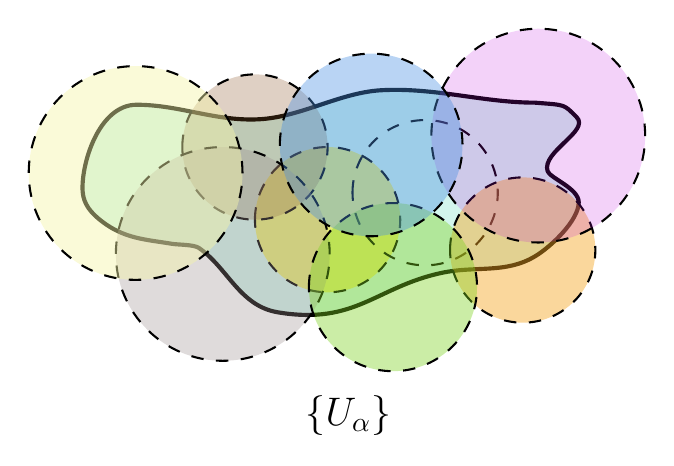
\begin{tikzpicture}[x=0.75pt,y=0.75pt,yscale=-1,xscale=1]
%uncomment if require: \path (0,227); %set diagram left start at 0, and has height of 227

%Curve Lines [id:da28281619681811754] 
\draw [fill={rgb, 255:red, 211; green, 245; blue, 236 }  ,fill opacity=1 ][line width=1.5] [line join = round][line cap = round]   (264,40.63) .. controls (239.07,40.63) and (216.02,33.24) .. (190,34.63) .. controls (169.94,35.71) and (151.25,47.57) .. (131,48.63) .. controls (109.98,49.74) and (92.57,41.63) .. (72,41.63) .. controls (53.59,41.63) and (45.01,70.73) .. (46,83.63) .. controls (46.47,89.7) and (50.18,93.88) .. (55,97.63) .. controls (66.08,106.25) and (76.24,106.51) .. (89,108.63) .. controls (91.95,109.13) and (99.58,108.96) .. (102,110.63) .. controls (115.88,120.24) and (121.56,138.56) .. (140,141.63) .. controls (177.55,147.89) and (187.14,129.46) .. (219,122.63) .. controls (235.52,119.09) and (249.69,123.22) .. (264,114.63) .. controls (271.71,110.01) and (285,97.32) .. (285,88.63) .. controls (285,81.9) and (271.1,76.94) .. (270,73.63) .. controls (266.91,64.36) and (290.59,54.22) .. (284,47.63) .. controls (277.54,41.17) and (279,41.85) .. (264,40.63) -- cycle ;
%Shape: Circle [id:dp001327175657310109] 
\draw  [fill={rgb, 255:red, 248; green, 231; blue, 28 }  ,fill opacity=0.55 ][dash pattern={on 4.5pt off 4.5pt}] (129,97) .. controls (129,77.67) and (144.67,62) .. (164,62) .. controls (183.33,62) and (199,77.67) .. (199,97) .. controls (199,116.33) and (183.33,132) .. (164,132) .. controls (144.67,132) and (129,116.33) .. (129,97) -- cycle ;
%Shape: Circle [id:dp7871419017635473] 
\draw  [dash pattern={on 4.5pt off 4.5pt}] (176,84) .. controls (176,64.67) and (191.67,49) .. (211,49) .. controls (230.33,49) and (246,64.67) .. (246,84) .. controls (246,103.33) and (230.33,119) .. (211,119) .. controls (191.67,119) and (176,103.33) .. (176,84) -- cycle ;
%Shape: Circle [id:dp8717686595013016] 
\draw  [fill={rgb, 255:red, 245; green, 166; blue, 35 }  ,fill opacity=0.45 ][dash pattern={on 4.5pt off 4.5pt}] (223,111.63) .. controls (223,92.3) and (238.67,76.63) .. (258,76.63) .. controls (277.33,76.63) and (293,92.3) .. (293,111.63) .. controls (293,130.96) and (277.33,146.63) .. (258,146.63) .. controls (238.67,146.63) and (223,130.96) .. (223,111.63) -- cycle ;
%Shape: Circle [id:dp9588061758851951] 
\draw  [fill={rgb, 255:red, 139; green, 87; blue, 42 }  ,fill opacity=0.28 ][dash pattern={on 4.5pt off 4.5pt}] (94,62) .. controls (94,42.67) and (109.67,27) .. (129,27) .. controls (148.33,27) and (164,42.67) .. (164,62) .. controls (164,81.33) and (148.33,97) .. (129,97) .. controls (109.67,97) and (94,81.33) .. (94,62) -- cycle ;
%Shape: Circle [id:dp9449595488988661] 
\draw  [fill={rgb, 255:red, 158; green, 145; blue, 145 }  ,fill opacity=0.33 ][dash pattern={on 4.5pt off 4.5pt}] (62,113.5) .. controls (62,85.06) and (85.06,62) .. (113.5,62) .. controls (141.94,62) and (165,85.06) .. (165,113.5) .. controls (165,141.94) and (141.94,165) .. (113.5,165) .. controls (85.06,165) and (62,141.94) .. (62,113.5) -- cycle ;
%Shape: Circle [id:dp5330131974534975] 
\draw  [fill={rgb, 255:red, 189; green, 16; blue, 224 }  ,fill opacity=0.19 ][dash pattern={on 4.5pt off 4.5pt}] (214,56.5) .. controls (214,28.06) and (237.06,5) .. (265.5,5) .. controls (293.94,5) and (317,28.06) .. (317,56.5) .. controls (317,84.94) and (293.94,108) .. (265.5,108) .. controls (237.06,108) and (214,84.94) .. (214,56.5) -- cycle ;
%Shape: Circle [id:dp4837000860245192] 
\draw  [fill={rgb, 255:red, 126; green, 211; blue, 33 }  ,fill opacity=0.4 ][dash pattern={on 4.5pt off 4.5pt}] (155,129.5) .. controls (155,107.13) and (173.13,89) .. (195.5,89) .. controls (217.87,89) and (236,107.13) .. (236,129.5) .. controls (236,151.87) and (217.87,170) .. (195.5,170) .. controls (173.13,170) and (155,151.87) .. (155,129.5) -- cycle ;
%Shape: Circle [id:dp17768072579265115] 
\draw  [fill={rgb, 255:red, 74; green, 144; blue, 226 }  ,fill opacity=0.39 ][dash pattern={on 4.5pt off 4.5pt}] (141,61) .. controls (141,36.7) and (160.7,17) .. (185,17) .. controls (209.3,17) and (229,36.7) .. (229,61) .. controls (229,85.3) and (209.3,105) .. (185,105) .. controls (160.7,105) and (141,85.3) .. (141,61) -- cycle ;
%Shape: Circle [id:dp406181221930618] 
\draw  [fill={rgb, 255:red, 244; green, 245; blue, 168 }  ,fill opacity=0.45 ][dash pattern={on 4.5pt off 4.5pt}] (20,74.5) .. controls (20,46.06) and (43.06,23) .. (71.5,23) .. controls (99.94,23) and (123,46.06) .. (123,74.5) .. controls (123,102.94) and (99.94,126) .. (71.5,126) .. controls (43.06,126) and (20,102.94) .. (20,74.5) -- cycle ;

% Text Node
\draw (152,180.4) node [anchor=north west][inner sep=0.75pt]  [font=\Large]  {$\{U_{\alpha }\}$};


\end{tikzpicture}

    \caption{Open cover of a space}
  \end{figure}
  \item \textit{Subspace Topology }is the topology on a subset $Y\subseteq X$ induced by the topology of $X$. In this case, open sets of $Y$ are basically the intersection of open sets of $X$ with $Y$. So,
  $$\uptau_Y = \{U\cap Y| U\in \uptau_X\}$$
  \end{itemize}
\subsection{Manifolds}
Let us see some pictures. 
\begin{figure}[H]
  \centering

  \begin{subfigure}[b]{0.3\textwidth}
    \centering
    

\tikzset{every picture/.style={line width=0.75pt}} %set default line width to 0.75pt        

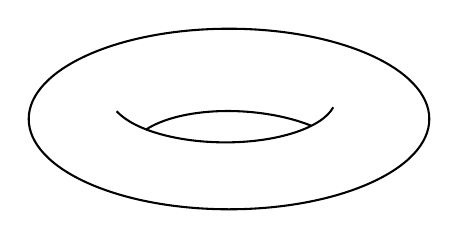
\begin{tikzpicture}[x=0.75pt,y=0.75pt,yscale=-1,xscale=1]
%uncomment if require: \path (0,300); %set diagram left start at 0, and has height of 300

%Shape: Ellipse [id:dp22801969143067424] 
\draw   (104,164.5) .. controls (104,140.48) and (147.2,121) .. (200.5,121) .. controls (253.8,121) and (297,140.48) .. (297,164.5) .. controls (297,188.52) and (253.8,208) .. (200.5,208) .. controls (147.2,208) and (104,188.52) .. (104,164.5) -- cycle ;
%Shape: Arc [id:dp10077529814620967] 
\draw  [draw opacity=0] (250.72,158.87) .. controls (245.28,168.82) and (223.36,176.06) .. (197.24,175.75) .. controls (173.88,175.48) and (154.02,169.25) .. (146.36,160.73) -- (197.5,153.5) -- cycle ; \draw   (250.72,158.87) .. controls (245.28,168.82) and (223.36,176.06) .. (197.24,175.75) .. controls (173.88,175.48) and (154.02,169.25) .. (146.36,160.73) ;  
%Shape: Arc [id:dp345385029103655] 
\draw  [draw opacity=0] (160.45,169.6) .. controls (170.37,163.16) and (188.19,159.59) .. (208.22,160.93) .. controls (220.26,161.74) and (231.27,164.2) .. (240.09,167.72) -- (206.61,184.82) -- cycle ; \draw   (160.45,169.6) .. controls (170.37,163.16) and (188.19,159.59) .. (208.22,160.93) .. controls (220.26,161.74) and (231.27,164.2) .. (240.09,167.72) ;  





\end{tikzpicture}

    \caption{Torus (yeah, donut came atlast!)}
  \end{subfigure}
  \hfill
  \begin{subfigure}[b]{0.3\textwidth}
    \centering
    

\tikzset{every picture/.style={line width=0.75pt}} %set default line width to 0.75pt        

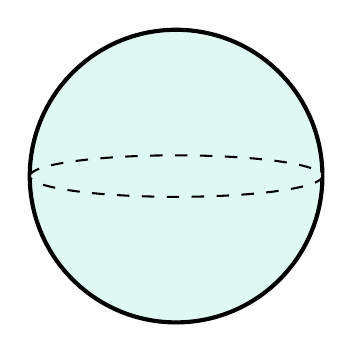
\begin{tikzpicture}[x=0.75pt,y=0.75pt,yscale=-1,xscale=1]
%uncomment if require: \path (0,300); %set diagram left start at 0, and has height of 300

%Shape: Circle [id:dp5828809729635696] 
\draw  [fill={rgb, 255:red, 223; green, 248; blue, 241 }  ,fill opacity=1 ][line width=1.5]  (161,152.5) .. controls (161,113.56) and (192.56,82) .. (231.5,82) .. controls (270.44,82) and (302,113.56) .. (302,152.5) .. controls (302,191.44) and (270.44,223) .. (231.5,223) .. controls (192.56,223) and (161,191.44) .. (161,152.5) -- cycle ;
%Shape: Ellipse [id:dp9903216585683989] 
\draw  [fill={rgb, 255:red, 223; green, 248; blue, 241 }  ,fill opacity=1 ][dash pattern={on 4.5pt off 4.5pt}] (161,152.5) .. controls (161,146.98) and (192.56,142.5) .. (231.5,142.5) .. controls (270.44,142.5) and (302,146.98) .. (302,152.5) .. controls (302,158.02) and (270.44,162.5) .. (231.5,162.5) .. controls (192.56,162.5) and (161,158.02) .. (161,152.5) -- cycle ;




\end{tikzpicture}

    \caption{Sphere (like yo mama)}
  \end{subfigure}
  \hfill
  \begin{subfigure}[b]{0.3\textwidth}
    \centering
    

\tikzset{every picture/.style={line width=0.75pt}} %set default line width to 0.75pt        

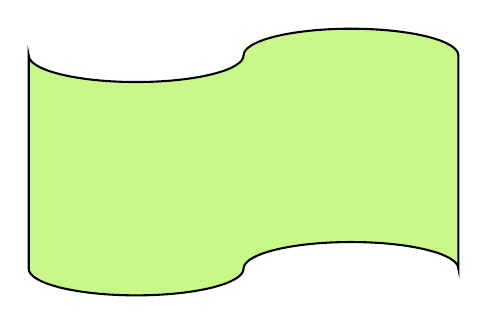
\begin{tikzpicture}[x=0.75pt,y=0.75pt,yscale=-1,xscale=1]
%uncomment if require: \path (0,300); %set diagram left start at 0, and has height of 300

%Flowchart: Punched Tape [id:dp25700721970086793] 
\draw  [fill={rgb, 255:red, 201; green, 248; blue, 137 }  ,fill opacity=1 ] (155,67.85) .. controls (155,74.94) and (178.17,80.69) .. (206.75,80.69) .. controls (235.33,80.69) and (258.5,74.94) .. (258.5,67.85) .. controls (258.5,60.75) and (281.67,55) .. (310.25,55) .. controls (338.83,55) and (362,60.75) .. (362,67.85) -- (362,170.62) .. controls (362,163.52) and (338.83,157.77) .. (310.25,157.77) .. controls (281.67,157.77) and (258.5,163.52) .. (258.5,170.62) .. controls (258.5,177.72) and (235.33,183.47) .. (206.75,183.47) .. controls (178.17,183.47) and (155,177.72) .. (155,170.62) -- cycle ;




\end{tikzpicture}

    \caption{A Waving Flag perhaps?}
  \end{subfigure}

  \caption{\textbf{What's common in all these?}}
\end{figure}
\noindent
So, what is common in all these pictures? Note that they all look very different from each other but if we really ZOOM in \emoji{mag-right} we can see that each of them look alike, like a \textit{flat plane}. Well, the road ahead of us looks flat but the road is on the freaking Earth which is, let's say to a physicist's satisfaction, a sphere. So, we can say that all of these things look `locally' like the flat plane $\mathbb{R}^2$. This is essentially the idea behind a \textbf{manifold}, things which look locally Euclidean (like $\mathbb{R}^n$). Let us define manifolds formally:
\begin{definition}[Manifold]
  $\mathcal{M}$ is a m-dimensional manifold if:
  \begin{itemize}
    \item $\mathcal{M}$ is a topological space.
    \item There exists an open cover $\{U_\alpha\}$ of $\mathcal{M}$ and for each $\alpha$, there exists a homeomorphism $\phi_\alpha: U_\alpha \to V_\alpha$ where $V_\alpha$ is an open subset of $\mathbb{R}^m$.
    \item Two open sets $U_i, U_j$ such that $U_i \cap U_j \neq \emptyset$, then the map $\psi_{ij} = \phi_i \circ \phi_j^{-1}$ is a smooth map \footnotemark, where $\psi_{ij}: \phi_j(U_i \cap U_j) \to \phi_i(U_i \cap U_j)$.
  \end{itemize}
\end{definition}
\footnotetext{
A smooth map is a function which is infinitely differentiable, that is, all the derivatives exist and are continuous. Sometimes a smooth map $f$ is said to belong to the class $C^\infty$. In general, $C^k$ is the class of functions which are $k$ times continuously differentiable. }
\begin{figure}[H]
  \centering 
  

% Pattern Info
 
\tikzset{
pattern size/.store in=\mcSize, 
pattern size = 5pt,
pattern thickness/.store in=\mcThickness, 
pattern thickness = 0.3pt,
pattern radius/.store in=\mcRadius, 
pattern radius = 1pt}
\makeatletter
\pgfutil@ifundefined{pgf@pattern@name@_z2kbg8xsc}{
\pgfdeclarepatternformonly[\mcThickness,\mcSize]{_z2kbg8xsc}
{\pgfqpoint{0pt}{0pt}}
{\pgfpoint{\mcSize+\mcThickness}{\mcSize+\mcThickness}}
{\pgfpoint{\mcSize}{\mcSize}}
{
\pgfsetcolor{\tikz@pattern@color}
\pgfsetlinewidth{\mcThickness}
\pgfpathmoveto{\pgfqpoint{0pt}{0pt}}
\pgfpathlineto{\pgfpoint{\mcSize+\mcThickness}{\mcSize+\mcThickness}}
\pgfusepath{stroke}
}}
\makeatother

% Pattern Info
 
\tikzset{
pattern size/.store in=\mcSize, 
pattern size = 5pt,
pattern thickness/.store in=\mcThickness, 
pattern thickness = 0.3pt,
pattern radius/.store in=\mcRadius, 
pattern radius = 1pt}
\makeatletter
\pgfutil@ifundefined{pgf@pattern@name@_gl41bao2a}{
\pgfdeclarepatternformonly[\mcThickness,\mcSize]{_gl41bao2a}
{\pgfqpoint{0pt}{0pt}}
{\pgfpoint{\mcSize+\mcThickness}{\mcSize+\mcThickness}}
{\pgfpoint{\mcSize}{\mcSize}}
{
\pgfsetcolor{\tikz@pattern@color}
\pgfsetlinewidth{\mcThickness}
\pgfpathmoveto{\pgfqpoint{0pt}{0pt}}
\pgfpathlineto{\pgfpoint{\mcSize+\mcThickness}{\mcSize+\mcThickness}}
\pgfusepath{stroke}
}}
\makeatother

% Pattern Info
 
\tikzset{
pattern size/.store in=\mcSize, 
pattern size = 5pt,
pattern thickness/.store in=\mcThickness, 
pattern thickness = 0.3pt,
pattern radius/.store in=\mcRadius, 
pattern radius = 1pt}
\makeatletter
\pgfutil@ifundefined{pgf@pattern@name@_uzph2v4rp}{
\pgfdeclarepatternformonly[\mcThickness,\mcSize]{_uzph2v4rp}
{\pgfqpoint{0pt}{0pt}}
{\pgfpoint{\mcSize+\mcThickness}{\mcSize+\mcThickness}}
{\pgfpoint{\mcSize}{\mcSize}}
{
\pgfsetcolor{\tikz@pattern@color}
\pgfsetlinewidth{\mcThickness}
\pgfpathmoveto{\pgfqpoint{0pt}{0pt}}
\pgfpathlineto{\pgfpoint{\mcSize+\mcThickness}{\mcSize+\mcThickness}}
\pgfusepath{stroke}
}}
\makeatother
\tikzset{every picture/.style={line width=0.75pt}} %set default line width to 0.75pt        

\begin{tikzpicture}[x=0.75pt,y=0.75pt,yscale=-1,xscale=1]
%uncomment if require: \path (0,351); %set diagram left start at 0, and has height of 351

%Curve Lines [id:da574442534870605] 
\draw [fill={rgb, 255:red, 211; green, 245; blue, 236 }  ,fill opacity=1 ][line width=1.5] [line join = round][line cap = round]   (359,39.63) .. controls (334.07,39.63) and (311.02,32.24) .. (285,33.63) .. controls (264.94,34.71) and (246.25,46.57) .. (226,47.63) .. controls (204.98,48.74) and (187.57,40.63) .. (167,40.63) .. controls (148.59,40.63) and (140.01,69.73) .. (141,82.63) .. controls (141.47,88.7) and (145.18,92.88) .. (150,96.63) .. controls (161.08,105.25) and (171.24,105.51) .. (184,107.63) .. controls (186.95,108.13) and (194.58,107.96) .. (197,109.63) .. controls (210.88,119.24) and (216.56,137.56) .. (235,140.63) .. controls (272.55,146.89) and (282.14,128.46) .. (314,121.63) .. controls (330.52,118.09) and (344.69,122.22) .. (359,113.63) .. controls (366.71,109.01) and (380,96.32) .. (380,87.63) .. controls (380,80.9) and (366.1,75.94) .. (365,72.63) .. controls (361.91,63.36) and (385.59,53.22) .. (379,46.63) .. controls (372.54,40.17) and (374,40.85) .. (359,39.63) -- cycle ;
%Shape: Circle [id:dp6828648905721534] 
\draw  [fill={rgb, 255:red, 248; green, 231; blue, 28 }  ,fill opacity=0.55 ][dash pattern={on 4.5pt off 4.5pt}] (205,87) .. controls (205,67.67) and (220.67,52) .. (240,52) .. controls (259.33,52) and (275,67.67) .. (275,87) .. controls (275,106.33) and (259.33,122) .. (240,122) .. controls (220.67,122) and (205,106.33) .. (205,87) -- cycle ;
%Shape: Circle [id:dp30983551895185024] 
\draw  [fill={rgb, 255:red, 189; green, 16; blue, 224 }  ,fill opacity=0.19 ][dash pattern={on 4.5pt off 4.5pt}] (252,82.5) .. controls (252,60.68) and (269.68,43) .. (291.5,43) .. controls (313.32,43) and (331,60.68) .. (331,82.5) .. controls (331,104.32) and (313.32,122) .. (291.5,122) .. controls (269.68,122) and (252,104.32) .. (252,82.5) -- cycle ;
%Shape: Path Data [id:dp349889120130531] 
\draw  [pattern=_z2kbg8xsc,pattern size=6pt,pattern thickness=0.75pt,pattern radius=0pt, pattern color={rgb, 255:red, 0; green, 0; blue, 0}][dash pattern={on 4.5pt off 4.5pt}] (275,87) .. controls (275,96.62) and (271.12,105.33) .. (264.85,111.65) .. controls (256.95,104.43) and (252,94.04) .. (252,82.5) .. controls (252,73.43) and (255.06,65.08) .. (260.19,58.41) .. controls (269.15,64.75) and (275,75.19) .. (275,87) -- cycle ;
%Straight Lines [id:da4063749285607826] 
\draw    (225,108) -- (187.94,177.58) ;
\draw [shift={(187,179.35)}, rotate = 298.04] [color={rgb, 255:red, 0; green, 0; blue, 0 }  ][line width=0.75]    (10.93,-3.29) .. controls (6.95,-1.4) and (3.31,-0.3) .. (0,0) .. controls (3.31,0.3) and (6.95,1.4) .. (10.93,3.29)   ;
%Straight Lines [id:da2660552290852516] 
\draw    (303,98) -- (347.96,171.64) ;
\draw [shift={(349,173.35)}, rotate = 238.6] [color={rgb, 255:red, 0; green, 0; blue, 0 }  ][line width=0.75]    (10.93,-3.29) .. controls (6.95,-1.4) and (3.31,-0.3) .. (0,0) .. controls (3.31,0.3) and (6.95,1.4) .. (10.93,3.29)   ;
% Consistent, clean axis arrows using TikZ arrow tips
\draw[->, line width=1] (132,266) -- (232,266); % x-axis
\draw[->, line width=1] (142,276) -- (142,176); % y-axis

\draw[->, line width=1] (314,266) -- (414,266); % x-axis
\draw[->, line width=1] (324,273) -- (324,173); % y-axis
%Shape: Circle [id:dp3856434949934364] 
\draw  [fill={rgb, 255:red, 184; green, 233; blue, 134 }  ,fill opacity=0.63 ][dash pattern={on 4.5pt off 4.5pt}] (156,223.5) .. controls (156,210.52) and (166.52,200) .. (179.5,200) .. controls (192.48,200) and (203,210.52) .. (203,223.5) .. controls (203,236.48) and (192.48,247) .. (179.5,247) .. controls (166.52,247) and (156,236.48) .. (156,223.5) -- cycle ;
%Shape: Circle [id:dp6236997602250793] 
\draw  [fill={rgb, 255:red, 245; green, 166; blue, 35 }  ,fill opacity=0.57 ][dash pattern={on 4.5pt off 4.5pt}] (338,217.5) .. controls (338,199) and (353,184) .. (371.5,184) .. controls (390,184) and (405,199) .. (405,217.5) .. controls (405,236) and (390,251) .. (371.5,251) .. controls (353,251) and (338,236) .. (338,217.5) -- cycle ;
%Shape: Path Data [id:dp5971497523670923] 
\draw  [pattern=_gl41bao2a,pattern size=6pt,pattern thickness=0.75pt,pattern radius=0pt, pattern color={rgb, 255:red, 0; green, 0; blue, 0}][dash pattern={on 4.5pt off 4.5pt}] (203,223.71) .. controls (203,231.18) and (199.04,237.95) .. (192.62,242.87) .. controls (184.56,237.25) and (179.5,229.18) .. (179.5,220.21) .. controls (179.5,213.16) and (182.62,206.67) .. (187.87,201.48) .. controls (197.02,206.41) and (203,214.53) .. (203,223.71) -- cycle ;
%Shape: Path Data [id:dp038898347866279326] 
\draw  [pattern=_uzph2v4rp,pattern size=6pt,pattern thickness=0.75pt,pattern radius=0pt, pattern color={rgb, 255:red, 0; green, 0; blue, 0}][dash pattern={on 4.5pt off 4.5pt}] (363,221.67) .. controls (363,230.57) and (358.79,238.64) .. (351.96,244.49) .. controls (343.38,237.81) and (338,228.19) .. (338,217.5) .. controls (338,209.1) and (341.32,201.37) .. (346.91,195.19) .. controls (356.64,201.06) and (363,210.73) .. (363,221.67) -- cycle ;
%Straight Lines [id:da8518964920780053] 
\draw [line width=1.5]    (350,223.02) -- (194,224) ;
\draw [shift={(191,224.02)}, rotate = 359.64] [color={rgb, 255:red, 0; green, 0; blue, 0 }  ][line width=1.5]    (14.21,-4.28) .. controls (9.04,-1.82) and (4.3,-0.39) .. (0,0) .. controls (4.3,0.39) and (9.04,1.82) .. (14.21,4.28)   ;

% Text Node
\draw (181,66.4) node [anchor=north west][inner sep=0.75pt]    {$U_{i}$};
% Text Node
\draw (332,58.4) node [anchor=north west][inner sep=0.75pt]    {$U_{j}$};
% Text Node
\draw (175,280.4) node [anchor=north west][inner sep=0.75pt]    {$\mathbb{R}^{m}$};
% Text Node
\draw (359,280.4) node [anchor=north west][inner sep=0.75pt]    {$\mathbb{R}^{m}$};
% Text Node
\draw (199,188.4) node [anchor=north west][inner sep=0.75pt]    {$U_{i} '$};
% Text Node
\draw (404,190.4) node [anchor=north west][inner sep=0.75pt]    {$U_{j} '$};
% Text Node
\draw (180,131.4) node [anchor=north west][inner sep=0.75pt]    {$\phi _{i}$};
% Text Node
\draw (339,131.4) node [anchor=north west][inner sep=0.75pt]    {$\phi _{j}$};
% Text Node
\draw (257,195.4) node [anchor=north west][inner sep=0.75pt]  [font=\large]  {$\psi _{i}{}_{j}$};
% Text Node
\draw (396,32.4) node [anchor=north west][inner sep=0.75pt]  [font=\Large]  {$\mathcal{M}$};


\end{tikzpicture}

  \caption{The figure shows the third point in the definition. So basically we see where the homeomorphism maps the intersection of the open sets and then define the map $\psi_{ij}$ between these two regions.}
\end{figure}
The terminologies used here are very much related to the geography of Earth. The pair $(U_i, \phi_i)$ is called a \textit{chart} (maybe because they help us to locally ``chart'' the manifold, that is, understand it using some coordinates) and the collection of all charts is called an \textit{atlas} (well, because it is collection of maps).\\[0.3cm]
Now let us unfold this carefully. For the open set $U_i$, the map $\phi_i$ takes it to another open set in $\mathbb{R}^m$. So for all $x\in U_i$ we got a mapping to an Euclidean space. Same goes for $U_j$, that is we obtain a mapping into another copy of $\mathbb{R}^m$. Now for points in the intersection of $U_i$ and $U_j$, we have got two different mappings and we can go back and forth between the two copies of $\mathbb{R}^m$ since these mappings were homeomorphisms. This is what we had with the mapping $\psi_{ij}$ (and thus, these are aptly called \textit{transition functions}). It first maps with the inverse of $\phi_j$  and then applies $\phi_i$. The net effect is that we are mapping between a point in one copy of $\mathbb{R}^m$ to another copy of $\mathbb{R}^m$. \\[0.3cm]
Imagine the open sets as patches in the manifold. We can then patch together the whole manifold by taking the union of all the open sets, all of which can be viewed as a Euclidean space. There are also manifolds which do not have the smooth property on then transient function, only continuity is required. These are called \textbf{topological manifolds}. We also assume that our manifolds are \textbf{Hausdorff} and paracompact (which we will not define here). Now comes the good thing: examples!!
\subsubsection{Examples:}
\textbf{The Space $\mathbf{\mathbb{R}^n}$}\\[0.3cm]
Duh, it looks like $\mathbb{R}^n$ locally since it is $\mathbb{R}^n$ itself. A single chart is enough for the purpose and the homeomorphism is the identity map. \\[0.3cm]
\textbf{The Circle $\mathbb{S}^1$}\\[0.3cm]
Circle is a curve in $\mathbb{R}^2$ with coordinates $(\cos\theta, \sin\theta)$. We mostly take $\theta \in [0,2\pi)$ but we come across a problem. Note that the open sets on a circle are basically union of ``open arcs''. However, $[0,2\pi)$ is not open. Thus we need atleast two charts to cover the circle.\\[0.3cm]
We take two antipodal points on the circle and then define the charts as follows: \\[0.3cm]
Let $U_1 = \mathbb{S}^1\backslash \{(1,0)\},U_2 = \mathbb{S}^1\backslash \{(-1,0)\}$. Then define the homeomorphisms as:
$$\phi_1: \mathbb{S}^1\backslash \{(1,0)\}\rightarrow (0,2\pi) \quad \quad \phi_2: \mathbb{S}^1\backslash \{(-1,0)\}\rightarrow (-\pi,\pi)$$
These functions basically take the value of the angle $\theta$ that a point on the circle makes with the x-axis.  
\begin{figure}[H]
  \centering
  \begin{subfigure}[b]{0.45\textwidth}
    \centering
    

\tikzset{every picture/.style={line width=0.75pt}} %set default line width to 0.75pt        

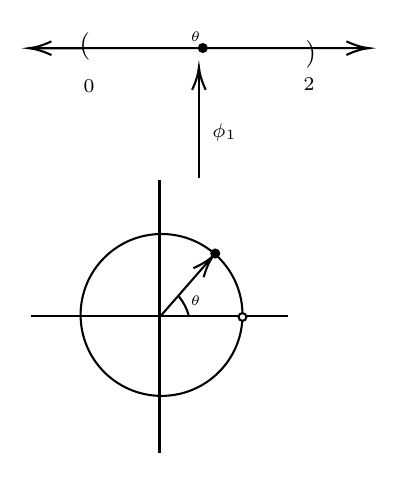
\begin{tikzpicture}[x=0.75pt,y=0.75pt,yscale=-1,xscale=1]
%uncomment if require: \path (0,300); %set diagram left start at 0, and has height of 300

\draw   (121,188.73) -- (245,188.73)(183,123) -- (183,254.47) ;
%Straight Lines [id:da8180273995647878] 
\draw    (122,59.5) -- (282,59.47) ;
\draw [shift={(284,59.47)}, rotate = 179.99] [color={rgb, 255:red, 0; green, 0; blue, 0 }  ][line width=0.75]    (10.93,-3.29) .. controls (6.95,-1.4) and (3.31,-0.3) .. (0,0) .. controls (3.31,0.3) and (6.95,1.4) .. (10.93,3.29)   ;
\draw [shift={(120,59.5)}, rotate = 359.99] [color={rgb, 255:red, 0; green, 0; blue, 0 }  ][line width=0.75]    (10.93,-3.29) .. controls (6.95,-1.4) and (3.31,-0.3) .. (0,0) .. controls (3.31,0.3) and (6.95,1.4) .. (10.93,3.29)   ;
%Shape: Circle [id:dp5128133772288312] 
\draw   (145,188) .. controls (145,166.46) and (162.46,149) .. (184,149) .. controls (205.54,149) and (223,166.46) .. (223,188) .. controls (223,209.54) and (205.54,227) .. (184,227) .. controls (162.46,227) and (145,209.54) .. (145,188) -- cycle ;
%Shape: Circle [id:dp8810895316002555] 
\draw  [fill={rgb, 255:red, 255; green, 255; blue, 255 }  ,fill opacity=1 ] (221.12,189) .. controls (221.12,187.96) and (221.96,187.12) .. (223,187.12) .. controls (224.04,187.12) and (224.88,187.96) .. (224.88,189) .. controls (224.88,190.04) and (224.04,190.88) .. (223,190.88) .. controls (221.96,190.88) and (221.12,190.04) .. (221.12,189) -- cycle ;
%Straight Lines [id:da9436577937186711] 
\draw    (184,188) -- (207.68,160.91) ;
\draw [shift={(209,159.4)}, rotate = 131.16] [color={rgb, 255:red, 0; green, 0; blue, 0 }  ][line width=0.75]    (10.93,-3.29) .. controls (6.95,-1.4) and (3.31,-0.3) .. (0,0) .. controls (3.31,0.3) and (6.95,1.4) .. (10.93,3.29)   ;
%Shape: Arc [id:dp6136432634457998] 
\draw  [draw opacity=0] (192.32,179.07) .. controls (194.56,181.78) and (196.24,184.99) .. (197.17,188.52) -- (174.15,194.94) -- cycle ; \draw   (192.32,179.07) .. controls (194.56,181.78) and (196.24,184.99) .. (197.17,188.52) ;  
%Straight Lines [id:da3473098561653878] 
\draw    (202,121.87) -- (202,70.62) ;
\draw [shift={(202,68.62)}, rotate = 90] [color={rgb, 255:red, 0; green, 0; blue, 0 }  ][line width=0.75]    (10.93,-3.29) .. controls (6.95,-1.4) and (3.31,-0.3) .. (0,0) .. controls (3.31,0.3) and (6.95,1.4) .. (10.93,3.29)   ;
%Shape: Circle [id:dp05894903245242711] 
\draw  [fill={rgb, 255:red, 0; green, 0; blue, 0 }  ,fill opacity=1 ] (208,158.4) .. controls (208,157.36) and (208.84,156.52) .. (209.88,156.52) .. controls (210.92,156.52) and (211.77,157.36) .. (211.77,158.4) .. controls (211.77,159.44) and (210.92,160.28) .. (209.88,160.28) .. controls (208.84,160.28) and (208,159.44) .. (208,158.4) -- cycle ;
%Shape: Circle [id:dp0797933236440207] 
\draw  [fill={rgb, 255:red, 0; green, 0; blue, 0 }  ,fill opacity=1 ] (202,59.4) .. controls (202,58.36) and (202.84,57.52) .. (203.88,57.52) .. controls (204.92,57.52) and (205.77,58.36) .. (205.77,59.4) .. controls (205.77,60.44) and (204.92,61.28) .. (203.88,61.28) .. controls (202.84,61.28) and (202,60.44) .. (202,59.4) -- cycle ;

% Text Node
\draw (196.5,177.1) node [anchor=north west][inner sep=0.75pt]  [font=\tiny]  {$\theta $};
% Text Node

% Text Node
\draw (142.88,50.5) node [anchor=north west][inner sep=0.75pt]  [rotate=-359.08]  {$($};
% Text Node
\draw (259.98,70.62) node [anchor=north west][inner sep=0.75pt]  [rotate=-180.17]  {$($};
% Text Node
\draw (144.88,73.5) node [anchor=north west][inner sep=0.75pt]  [font=\scriptsize,rotate=-359.08]  {$0$};
% Text Node
\draw (250.88,72.5) node [anchor=north west][inner sep=0.75pt]  [font=\scriptsize,rotate=-359.08]  {$2\uppi $};
% Text Node
\draw (196.5,50.1) node [anchor=north west][inner sep=0.75pt]  [font=\tiny]  {$\theta $};
% Text Node
\draw (206.88,94.5) node [anchor=north west][inner sep=0.75pt]  [font=\scriptsize,rotate=-359.08]  {$\phi _{1}$};


\end{tikzpicture}

    \caption{Here the point $(1,0)$ is removed and $\phi_1$ maps the rest of the circle to the interval $(0,2\pi)$.}
    \label{fig:circchart1}
  \end{subfigure}
  \hfill
  \begin{subfigure}[b]{0.45\textwidth}
    \centering
    

\tikzset{every picture/.style={line width=0.75pt}} %set default line width to 0.75pt        

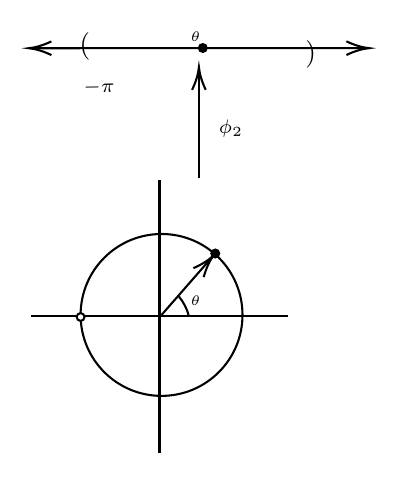
\begin{tikzpicture}[x=0.75pt,y=0.75pt,yscale=-1,xscale=1]
%uncomment if require: \path (0,300); %set diagram left start at 0, and has height of 300

\draw   (258,177.73) -- (382,177.73)(320,112) -- (320,243.47) ;
%Straight Lines [id:da1268514518445265] 
\draw    (259,48.5) -- (419,48.47) ;
\draw [shift={(421,48.47)}, rotate = 179.99] [color={rgb, 255:red, 0; green, 0; blue, 0 }  ][line width=0.75]    (10.93,-3.29) .. controls (6.95,-1.4) and (3.31,-0.3) .. (0,0) .. controls (3.31,0.3) and (6.95,1.4) .. (10.93,3.29)   ;
\draw [shift={(257,48.5)}, rotate = 359.99] [color={rgb, 255:red, 0; green, 0; blue, 0 }  ][line width=0.75]    (10.93,-3.29) .. controls (6.95,-1.4) and (3.31,-0.3) .. (0,0) .. controls (3.31,0.3) and (6.95,1.4) .. (10.93,3.29)   ;
%Shape: Circle [id:dp7024113415149893] 
\draw   (282,177) .. controls (282,155.46) and (299.46,138) .. (321,138) .. controls (342.54,138) and (360,155.46) .. (360,177) .. controls (360,198.54) and (342.54,216) .. (321,216) .. controls (299.46,216) and (282,198.54) .. (282,177) -- cycle ;
%Shape: Circle [id:dp9335574434248441] 
\draw  [fill={rgb, 255:red, 255; green, 255; blue, 255 }  ,fill opacity=1 ] (280.12,178) .. controls (280.12,176.96) and (280.96,176.12) .. (282,176.12) .. controls (283.04,176.12) and (283.88,176.96) .. (283.88,178) .. controls (283.88,179.04) and (283.04,179.88) .. (282,179.88) .. controls (280.96,179.88) and (280.12,179.04) .. (280.12,178) -- cycle ;
%Straight Lines [id:da8252578804556748] 
\draw    (321,177) -- (344.68,149.91) ;
\draw [shift={(346,148.4)}, rotate = 131.16] [color={rgb, 255:red, 0; green, 0; blue, 0 }  ][line width=0.75]    (10.93,-3.29) .. controls (6.95,-1.4) and (3.31,-0.3) .. (0,0) .. controls (3.31,0.3) and (6.95,1.4) .. (10.93,3.29)   ;
%Shape: Arc [id:dp3291144774774024] 
\draw  [draw opacity=0] (329.32,168.07) .. controls (331.56,170.78) and (333.24,173.99) .. (334.17,177.52) -- (311.15,183.94) -- cycle ; \draw   (329.32,168.07) .. controls (331.56,170.78) and (333.24,173.99) .. (334.17,177.52) ;  
%Straight Lines [id:da3615704984807794] 
\draw    (339,110.87) -- (339,59.62) ;
\draw [shift={(339,57.62)}, rotate = 90] [color={rgb, 255:red, 0; green, 0; blue, 0 }  ][line width=0.75]    (10.93,-3.29) .. controls (6.95,-1.4) and (3.31,-0.3) .. (0,0) .. controls (3.31,0.3) and (6.95,1.4) .. (10.93,3.29)   ;
%Shape: Circle [id:dp19768643904648886] 
\draw  [fill={rgb, 255:red, 0; green, 0; blue, 0 }  ,fill opacity=1 ] (345,147.4) .. controls (345,146.36) and (345.84,145.52) .. (346.88,145.52) .. controls (347.92,145.52) and (348.77,146.36) .. (348.77,147.4) .. controls (348.77,148.44) and (347.92,149.28) .. (346.88,149.28) .. controls (345.84,149.28) and (345,148.44) .. (345,147.4) -- cycle ;
%Shape: Circle [id:dp2589693685269747] 
\draw  [fill={rgb, 255:red, 0; green, 0; blue, 0 }  ,fill opacity=1 ] (339,48.4) .. controls (339,47.36) and (339.84,46.52) .. (340.88,46.52) .. controls (341.92,46.52) and (342.77,47.36) .. (342.77,48.4) .. controls (342.77,49.44) and (341.92,50.28) .. (340.88,50.28) .. controls (339.84,50.28) and (339,49.44) .. (339,48.4) -- cycle ;

% Text Node
\draw (333.5,166.1) node [anchor=north west][inner sep=0.75pt]  [font=\tiny]  {$\theta $};
% Text Node

% Text Node
\draw (279.88,39.5) node [anchor=north west][inner sep=0.75pt]  [rotate=-359.08]  {$($};
% Text Node
\draw (396.98,59.62) node [anchor=north west][inner sep=0.75pt]  [rotate=-180.17]  {$($};
% Text Node
\draw (281.88,62.5) node [anchor=north west][inner sep=0.75pt]  [font=\scriptsize,rotate=-359.08]  {$-\pi $};
% Text Node
\draw (387.88,61.5) node [anchor=north west][inner sep=0.75pt]  [font=\scriptsize,rotate=-359.08]  {$\uppi $};
% Text Node
\draw (333.5,39.1) node [anchor=north west][inner sep=0.75pt]  [font=\tiny]  {$\theta $};
% Text Node
\draw (347.05,81.61) node [anchor=north west][inner sep=0.75pt]  [font=\scriptsize,rotate=-359.08]  {$\phi _{2}$};


\end{tikzpicture}

    \caption{Here the point $(-1,0)$ is removed and $\phi_2$ maps the rest of the circle to the interval $(-\pi,\pi)$.}
    \label{fig:circchart2}
  \end{subfigure}
  \caption{$\phi_1$ and $\phi_2$ are invertiable and continuous (easily seen).  The two charts intersect in the upper and lower semicircles (as the antipodal points are removed). The transition function is given by:
  \(\phi_1 \circ \phi_2^{-1}(\theta) = \begin{cases}   \theta  & \text{if } \theta\in (0, \pi) \\  \theta+2\pi & \text{if } \theta \in (-\pi, 0) \end{cases}\)which is \textit{smooth} on each of the semicircles as required. Thus this is a valid chart for the circle.}  
  
\end{figure}
\noindent
The same circle can be described by another chart using the stereographic projection, resulting in the \textbf{Mercator Atlas}. \textcolor{red}{show this maybe}..
Similarly we can prove that the $n$-dimensional sphere is a manifold. \\[0.3cm]
\textbf{Product Manifold:}\\[0.2cm]
Let $\mathcal{M}$ be an $m$-dimensional manifold with atlas $\{U_i,\phi_i\}$ and $\mathcal{N}$ be an $n$-dimensional manifold with atlas $\{V_i,\psi_i\}$, then we define the product manifold as an $(m+n)-$ dimensional manifold with atlas $\{U_i\times V_j, (\phi_i\, \psi_j)\}$. So basically we took the Cartesian product of the two coordinate neighbourhoods to define the new neighbourhood and then used the ordered pair of the two homeomorphisms to define the new coordinate function. \\[0.3cm]
\textit{Example.} The torus is a product manifold of two circles, that is, $T^2 = \mathbb{S}^1\times \mathbb{S}^1$. Note that by our definition, it is a two $(1+1)$ dimensional manifold. We can generalise the notion of torus by taking multiple product of circles: $$T^n = \underbrace{\mathbb{S}^1\times \mathbb{S}^1\times \cdots \times \mathbb{S}^1}_n$$ 
\subsubsection{Differentiable Maps}
\begin{definition}[Differentiable Map]
  Let $f: \mathcal{M}_m \to \mathcal{N}_n$ be a map between two manifolds such that $p\in M, p \mapsto f(p)\in N$
\end{definition}
\subsection{Tangent Spaces}
\subsection{Differential Forms}
% \textit{Definition.} Suppose $C\subset \mathbb{R}^2$ be a curve and let $p\in C$ is a point. The tangent space to $C$ at $p$ is the set of all vectors tangent to $C$ at $p$ and is denoted by $T_pC$. 